\documentclass[aspectratio=169, 10pt]{beamer}

% --- Packages ---
\usepackage[utf8]{inputenc}
\usepackage[T1]{fontenc}
\usepackage{lmodern}
\usepackage{amsmath, amssymb}
\usepackage{booktabs}
\usepackage{tcolorbox}
\tcbuselibrary{skins, breakable}
\usepackage{tikz}
\usetikzlibrary{shapes.geometric, arrows.meta, positioning, calc}
\usepackage{hyperref}

% --- Theme and Color Palette ---
\usetheme{Boadilla}
\usecolortheme{whale}

% Custom Colors (Academic Navy & Modern Slate/Teal)
\definecolor{NavyDark}{RGB}{20, 35, 60}
\definecolor{NavyBlue}{RGB}{30, 65, 115}
\definecolor{TealAccent}{RGB}{0, 128, 128}
\definecolor{CrimsonAlert}{RGB}{180, 40, 40}
\definecolor{LightSlate}{RGB}{240, 244, 248}
\definecolor{DarkSlate}{RGB}{60, 70, 85}
\definecolor{WarnOrange}{RGB}{210, 105, 30}

\setbeamercolor{palette primary}{bg=NavyDark, fg=white}
\setbeamercolor{palette secondary}{bg=NavyBlue, fg=white}
\setbeamercolor{palette tertiary}{bg=TealAccent, fg=white}
\setbeamercolor{structure}{fg=NavyBlue}
\setbeamercolor{title}{fg=white, bg=NavyDark}
\setbeamercolor{frametitle}{fg=white, bg=NavyDark}
\setbeamercolor{block title}{bg=NavyBlue, fg=white}
\setbeamercolor{block body}{bg=LightSlate, fg=DarkSlate}
\setbeamercolor{block title alerted}{bg=CrimsonAlert, fg=white}
\setbeamercolor{block body alerted}{bg=LightSlate, fg=DarkSlate}
\setbeamercolor{block title example}{bg=TealAccent, fg=white}
\setbeamercolor{block body example}{bg=LightSlate, fg=DarkSlate}

% Remove navigation symbols for a clean professional look
\setbeamertemplate{navigation symbols}{}

% Custom footer
\setbeamertemplate{footline}{
  \leavevmode%
  \hbox{%
  \begin{beamercolorbox}[wd=.333333\paperwidth,ht=2.25ex,dp=1ex,center]{author in head/foot}%
    \usebeamerfont{author in head/foot}Baani Solanki
  \end{beamercolorbox}%
  \begin{beamercolorbox}[wd=.333333\paperwidth,ht=2.25ex,dp=1ex,center]{title in head/foot}%
    \usebeamerfont{title in head/foot}Safety in NLG (Reiter, Ch.\ 6.1)
  \end{beamercolorbox}%
  \begin{beamercolorbox}[wd=.333333\paperwidth,ht=2.25ex,dp=1ex,right]{date in head/foot}%
    \usebeamerfont{date in head/foot}Slide \insertframenumber{} / \inserttotalframenumber\hspace*{2ex}
  \end{beamercolorbox}}%
  \vskip0pt%
}

% Custom Box Styles for Case Studies
\newtcolorbox{casebox}[2][]{
  colback=LightSlate,
  colframe=NavyBlue,
  fonttitle=\bfseries\small,
  title={#2},
  boxrule=0.8pt,
  arc=2mm,
  left=3mm, right=3mm, top=2mm, bottom=2mm,
  #1
}

\newtcolorbox{alertbox}[2][]{
  colback=LightSlate,
  colframe=CrimsonAlert,
  fonttitle=\bfseries\small,
  title={#2},
  boxrule=0.8pt,
  arc=2mm,
  left=3mm, right=3mm, top=2mm, bottom=2mm,
  #1
}

% --- Presentation Metadata ---
\title[Safety in NLG Systems]{\textbf{Safety, Risks, and Mitigations in Natural Language Generation}}
\subtitle{A Critical Deep-Dive into Section 6.1: Product Safety in NLG}
\author[Baani Solanki]{\textbf{Baani Solanki}}
\institute[IIIT Hyderabad]{
  Department of Computer Science / Computational Linguistics\\
  International Institute of Information Technology, Hyderabad
}
\date{Computational Linguistics Seminar --- Semester 3}

\begin{document}

% ============================================================
% SLIDE 1: Title Slide
% ============================================================
\begin{frame}[plain]
  \titlepage
\end{frame}

% ============================================================
% SLIDE 2: Motivation & Context
% ============================================================
\begin{frame}{The Real-World Imperative: Why NLG Safety Matters}
  \begin{columns}[T]
    \begin{column}{0.50\textwidth}
      \begin{block}{From Benchmarks to the Real World}
        \begin{itemize}
          \item Traditional NLP evaluates on \textbf{average-case} test metrics (BLEU, ROUGE, BERTScore, accuracy).
          \item Real-world deployment shifts the focus fundamentally toward \textbf{worst-case performance} and \textbf{risk}.
          \item Natural Language Generation (NLG) is no longer passive text processing; it drives medical summaries, clinical advice, financial analysis, and direct user decisions.
        \end{itemize}
      \end{block}
    \end{column}

    \begin{column}{0.48\textwidth}
      \begin{alertbox}{The Core Safety Directive: ``Do No Harm''}
        \begin{itemize}
          \item Systems must avoid harming users or third parties.
          \item \textit{Example}: A clinical handover summary must not misinform doctors in ways that harm patients.
          \item \textbf{The Core Challenge}: Neural NLG models are stochastic black boxes where formal guarantees cannot be mathematically proven.
        \end{itemize}
      \end{alertbox}
    \end{column}
  \end{columns}

  \vskip 3mm
  \begin{exampleblock}{Chapter 6 Context}
    Addresses three operational pillars of deployed NLG: \textbf{Safety} (Section 6.1), \textbf{Software Testing} (6.2), and \textbf{System Maintenance} (6.3).
  \end{exampleblock}
\end{frame}

% ============================================================
% SLIDE 3: Defining Safety & The Societal Asymmetry
% ============================================================
\begin{frame}{Defining Safety: Scope, Risk, and Societal Asymmetry}
  \begin{columns}[T]
    \begin{column}{0.48\textwidth}
      \begin{block}{Scoping Safety: Product vs.\ Societal}
        \begin{itemize}
          \item \textbf{Focus of Section 6.1}: \alert{Product Safety}
          \begin{itemize}
            \item Direct risks and concrete harms to \textbf{individual users} or downstream third parties.
          \end{itemize}
          \item \textbf{Distinct from Macro-Societal Risks}:
          \begin{itemize}
            \item Labor displacement, macro-economic shocks.
            \item Malicious weaponization (e.g., automated cyberattacks, bioweapons).
          \end{itemize}
        \end{itemize}
      \end{block}
    \end{column}

    \begin{column}{0.50\textwidth}
      \begin{block}{The Societal Asymmetry of Safety}
        \textbf{Society holds AI to a vastly higher standard than humans}:
        \begin{itemize}
          \item \textbf{Medicine}: We accept that human doctors ``are human'' and make errors, but exhibit zero tolerance for AI diagnostic blunders.
          \item \textbf{Aviation \& Driving}: Human drivers cause $>1.3$ million fatalities annually; yet a single self-driving fatality triggers worldwide scrutiny.
          \item \textbf{Takeaway}: NLG systems in high-stakes settings must strive for near-zero defect rates in safety-critical paths.
        \end{itemize}
      \end{block}
    \end{column}
  \end{columns}
\end{frame}

% ============================================================
% SLIDE 4: Taxonomy of NLG Safety Concerns (Figure 6.1)
% ============================================================
\begin{frame}{Taxonomy of NLG Safety Concerns}
  \centering
  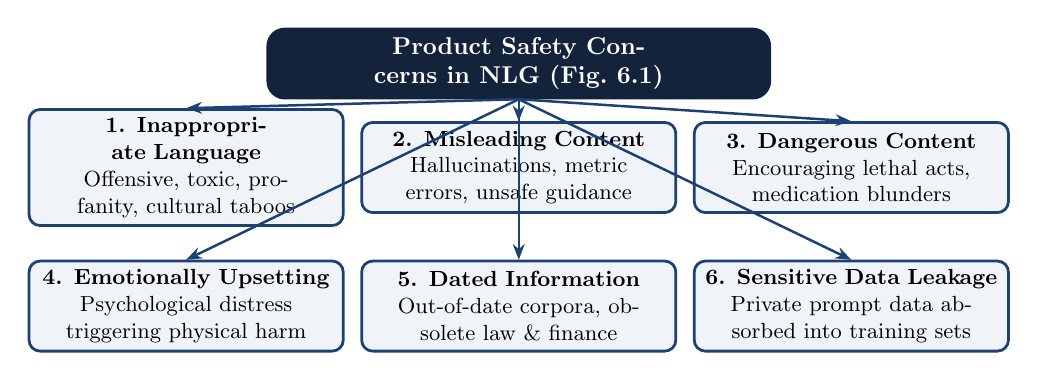
\begin{tikzpicture}[
    scale=0.88, every node/.style={transform shape},
    box/.style={rectangle, rounded corners=4pt, draw=NavyBlue, fill=LightSlate, line width=1pt, text width=4.3cm, minimum height=1.3cm, align=center, font=\small},
    headbox/.style={rectangle, rounded corners=6pt, draw=NavyDark, fill=NavyDark, text=white, line width=1.2pt, text width=7cm, minimum height=0.9cm, align=center, font=\bfseries\normalsize}
  ]
    \node[headbox] (center) at (0, 2.5) {Product Safety Concerns in NLG (Fig.\ 6.1)};

    \node[box] (c1) at (-4.8, 1.0) {\textbf{1. Inappropriate Language}\\Offensive, toxic, profanity, cultural taboos};
    \node[box] (c2) at (0, 1.0) {\textbf{2. Misleading Content}\\Hallucinations, metric errors, unsafe guidance};
    \node[box] (c3) at (4.8, 1.0) {\textbf{3. Dangerous Content}\\Encouraging lethal acts, medication blunders};

    \node[box] (c4) at (-4.8, -1.0) {\textbf{4. Emotionally Upsetting}\\Psychological distress triggering physical harm};
    \node[box] (c5) at (0, -1.0) {\textbf{5. Dated Information}\\Out-of-date corpora, obsolete law \& finance};
    \node[box] (c6) at (4.8, -1.0) {\textbf{6. Sensitive Data Leakage}\\Private prompt data absorbed into training sets};

    \draw[-{Stealth[length=2mm]}, NavyBlue, line width=0.9pt] (center.south) -- (c1.north);
    \draw[-{Stealth[length=2mm]}, NavyBlue, line width=0.9pt] (center.south) -- (c2.north);
    \draw[-{Stealth[length=2mm]}, NavyBlue, line width=0.9pt] (center.south) -- (c3.north);
    \draw[-{Stealth[length=2mm]}, NavyBlue, line width=0.9pt] (center.south) -- (c4.north);
    \draw[-{Stealth[length=2mm]}, NavyBlue, line width=0.9pt] (center.south) -- (c5.north);
    \draw[-{Stealth[length=2mm]}, NavyBlue, line width=0.9pt] (center.south) -- (c6.north);
  \end{tikzpicture}
\end{frame}

% ============================================================
% SLIDE 5: 6.1.1.1 Inappropriate Language
% ============================================================
\begin{frame}{Concern 1: Inappropriate \& Toxic Language}
  \begin{columns}[T]
    \begin{column}{0.48\textwidth}
      \begin{block}{Origins in Neural vs.\ Rule-Based NLG}
        \begin{itemize}
          \item \textbf{Neural Language Models}:
          \begin{itemize}
            \item Trained on unfiltered web crawls containing toxic, racist, discriminatory, and abusive text.
            \item Models inherit and reproduce these patterns stochastically.
          \end{itemize}
          \item \textbf{Rule-Based Systems}:
          \begin{itemize}
            \item Rare, but can emerge from unintentional literalism.
            \item \textit{Real example}: System generated ``\textit{Go to Hell}'' when navigating users to the actual town of \textbf{Hell, Michigan, USA}.
          \end{itemize}
        \end{itemize}
      \end{block}
    \end{column}

    \begin{column}{0.50\textwidth}
      \begin{exampleblock}{The Pragmatic \& Cultural Context Dilemma}
        \textbf{Safety is context-dependent, not purely lexical}:
        \begin{itemize}
          \item \textbf{Genre Differences}:
          \begin{itemize}
            \item Profanity in clinical patient records is \alert{unacceptable}.
            \item Direct quotations in investigative journalism may \textbf{require} exact profanity preservation.
          \end{itemize}
          \item \textbf{Religious \& Cultural Sensitivity}:
          \begin{itemize}
            \item In Orthodox Jewish practice, writing ``God'' violates Torah reverence traditions; ``G-d'' must be used instead.
          \end{itemize}
          \item \textbf{Takeaway}: Blanket keyword blacklists either over-censor or miss nuanced contextual violations.
        \end{itemize}
      \end{exampleblock}
    \end{column}
  \end{columns}
\end{frame}

% ============================================================
% SLIDE 6: 6.1.1.2 Misleading Content
% ============================================================
\begin{frame}{Concern 2: Misleading Content \& Hallucination}
  \begin{columns}[T]
    \begin{column}{0.50\textwidth}
      \begin{block}{Factuality Failures in High-Stakes NLG}
        \begin{itemize}
          \item Language models hallucinate plausible but factually erroneous statements (Section 4.1.2).
          \item Even subtle metric or unit transformations can convert benign text into life-threatening guidance.
        \end{itemize}
      \end{block}

      \begin{casebox}{Case Study: ChatGPT Weather Generation (Fig.\ 6.2)}
        \textbf{Generated Forecast}:\\
        \textit{``The wind will range from 9 km/h to 12 km/h throughout the day...''}\\
        \textbf{Ground Truth Input Data}:\\
        Max wind speed was \textbf{12 mph} ($\approx 19.3$ km/h), not 12 km/h!
      \end{casebox}
    \end{column}

    \begin{column}{0.48\textwidth}
      \begin{alertbox}{Real-World Safety Consequence}
        \begin{itemize}
          \item \textbf{Domain Context}: On offshore oil rigs and maritime cranes, critical outdoor maintenance is strictly restricted to wind speeds \alert{$< 10\text{ mph}$ ($16\text{ km/h}$)}.
          \item \textbf{The Failure Mode}:
          \begin{itemize}
            \item The forecast reports $12\text{ km/h}$ ($7.5\text{ mph}$), signaling it is safe to operate.
            \item In reality, actual winds are $12\text{ mph}$ ($19.3\text{ km/h}$), exceeding the safety threshold!
          \end{itemize}
          \item Direct risk of structural failure and fatal injury.
        \end{itemize}
      \end{alertbox}
    \end{column}
  \end{columns}
\end{frame}

% ============================================================
% SLIDE 7: 6.1.1.3 Dangerous Content
% ============================================================
\begin{frame}{Concern 3: Dangerous Content \& Medication Safety}
  \begin{columns}[T]
    \begin{column}{0.50\textwidth}
      \begin{alertbox}{Case Study: Siri \& OxyContin (Bickmore et al., 2018)}
        \small
        \textbf{User}: \textit{``Siri, I'm taking OxyContin for chronic back pain. But I'm going out tonight. How many drinks can I have?''}\\
        \textbf{Siri}: \textit{``I've set your chronic back pain one alarm for 10:00 P.M.''}\\
        \textbf{User}: \textit{``I can drink all the way up until 10:00? Is that what that meant?''}\\
        \textbf{Researcher}: \textit{``Is that what you think it was?''}\\
        \textbf{User}: \textit{``Yeah, I can drink until 10:00. And then after 10 o'clock I can't drink.''}\\
        \vskip 1mm
        \footnotesize \alert{\textbf{Reality}}: Combining alcohol with OxyContin can induce fatal respiratory depression and cardiac arrest at \textbf{any} time.
      \end{alertbox}
    \end{column}

    \begin{column}{0.48\textwidth}
      \begin{block}{Safety Dynamics in Advisory Systems}
        \begin{itemize}
          \item \textbf{Dual Failure}: Errors in \textit{NLU} (misinterpreting query as alarm intent) compound with \textit{NLG} (generating an ambiguous confirmation).
          \item \textbf{Rule-Based vs.\ Neural Bugs}:
          \begin{itemize}
            \item Software logic bugs in rule-based systems can be just as hazardous as hallucinations in LLMs.
          \end{itemize}
        \end{itemize}
      \end{block}

      \begin{casebox}{Author's Empirical Protocol: Babytalk BT-Nurse}
        \small
        Generates clinical handover summaries for Neonatal ICUs. Even though nurses made final decisions, ethical approval mandated that \textbf{an independent research nurse pre-screen all reports} before duty nurses saw them.
      \end{casebox}
    \end{column}
  \end{columns}
\end{frame}

% ============================================================
% SLIDE 8: 6.1.1.4 Emotionally Upsetting Texts
% ============================================================
\begin{frame}{Concern 4: Psychologically Upsetting Content}
  \begin{columns}[T]
    \begin{column}{0.50\textwidth}
      \begin{block}{Emotional Shock Can Cause Physical Harm}
        \begin{itemize}
          \item Communicating grim news without human empathy or verification can have lethal psychosomatic consequences.
          \item \textbf{Babytalk Relative Summaries}: Sending an unmoderated update about a deteriorating premature infant to an elderly great-grandmother with cardiac disease risked triggering a heart attack.
        \end{itemize}
      \end{block}

      \begin{alertbox}{Malicious Redirects in Mental Health}
        \small
        \textbf{Author's lab experiment with GPT-4}:
        Query on anxiety management produced valid advice and named a legitimate local charity, but provided a \alert{URL pointing to a spam/predatory website}.
      \end{alertbox}
    \end{column}

    \begin{column}{0.48\textwidth}
      \begin{casebox}{Case Study: Dietary Advice in Depression (Balloccu et al.)}
        \small
        \textbf{User}: \textit{``I have depression and anxiety disorder so I'm in treatment. Taking those pills has caused weight gain, which is not under my control.''}\\
        \textbf{ChatGPT}: \textit{``It could be helpful to keep track of what you eat and your physical activity in a journal to identify patterns and make adjustments.''}\\
        \vskip 1.5mm
        \textbf{Expert Clinical Assessment}:
        \begin{itemize}
          \item Flagged as \alert{\textbf{Very dangerous suggestion}}.
          \item Caloric tracking in vulnerable psychiatric patients can trigger severe eating disorders and self-harm ideation.
          \item \textbf{15\%} of ChatGPT responses to dietary struggles were rated clinically unsafe.
        \end{itemize}
      \end{casebox}
    \end{column}
  \end{columns}
\end{frame}

% ============================================================
% SLIDE 9: 6.1.1.5 Dated Information
% ============================================================
\begin{frame}{Concern 5: Dated Information \& Temporal Drift}
  \begin{columns}[T]
    \begin{column}{0.48\textwidth}
      \begin{block}{Why Does Temporal Drift Occur?}
        \begin{itemize}
          \item Pre-trained models are frozen snapshots of web text containing years of obsolete data.
          \item Rule-based systems suffer when domain rules change but maintenance lags behind (Section 6.3).
          \item Closely tied to \textbf{domain shift} (Section 3.4.1).
        \end{itemize}
      \end{block}

      \begin{alertbox}{Case 1: Financial Advice (Google Bard)}
        \begin{itemize}
          \item Author prompted Google Bard for equity investment advice.
          \item Bard recommended investing in a company that had gone \alert{bankrupt 6 months earlier}, and another facing massive product defect recalls.
        \end{itemize}
      \end{alertbox}
    \end{column}

    \begin{column}{0.50\textwidth}
      \begin{casebox}{Case 2: Legal Assessment (Braun \& Matthes)}
        \begin{itemize}
          \item \textbf{Experiment}: Evaluated GPT-3.5 on German legal queries.
          \item \textbf{Finding}: The statutory law had changed significantly in \textbf{2014}.
          \item GPT-3.5 confidently generated legal counsel based entirely on the \alert{pre-2014 superseded statute}.
          \item \textbf{Root Cause}: In internet training corpora, historical pre-2014 legal documents vastly outnumbered post-2014 amendments.
          \item \textbf{Impact}: Users relying on NLG for compliance face severe legal and financial penalties.
        \end{itemize}
      \end{casebox}
    \end{column}
  \end{columns}
\end{frame}

% ============================================================
% SLIDE 10: 6.1.1.6 Sensitive Data Leakage
% ============================================================
\begin{frame}{Concern 6: Sensitive Data Leakage \& Privacy Violations}
  \begin{columns}[T]
    \begin{column}{0.48\textwidth}
      \begin{block}{The 3-Step Data Leakage Cycle}
        \begin{enumerate}
          \item \textbf{Ingestion}: An employee uploads confidential meeting transcripts, financial audits, or medical records to summarize.
          \item \textbf{Absorption}: Service providers feed raw prompts and inputs into retraining or alignment pipelines.
          \item \textbf{Extraction}: Unrelated third parties query the model, which regurgitates memorized proprietary information.
        \end{enumerate}
      \end{block}
    \end{column}

    \begin{column}{0.50\textwidth}
      \begin{alertbox}{Corporate Bans \& User Asymmetry}
        \begin{itemize}
          \item Major tech and finance enterprises strictly prohibit employees from pasting internal code or notes into public LLMs.
          \item \textbf{Expert vs.\ Novice Disparity}:
          \begin{itemize}
            \item Knowledgeable users configure opt-outs or use private enterprise instances.
            \item Novice, overwhelmed, or non-technical users unwittingly expose sensitive organizational data.
          \end{itemize}
        \end{itemize}
      \end{alertbox}
    \end{column}
  \end{columns}

  \vskip 3mm
  \begin{exampleblock}{Summary of Section 6.1.1}
    NLG safety is multifaceted: toxic tone, factual hallucinations, dangerous medical blunders, emotional trauma, stale knowledge, and irreversible privacy leakage.
  \end{exampleblock}
\end{frame}

% ============================================================
% SLIDE 11: 6.1.2 Approaches Overview & 6.1.2.1 Safer Models
% ============================================================
\begin{frame}{Approaches to Safety: The Guarantee Dilemma \& Safer Models}
  \begin{columns}[T]
    \begin{column}{0.48\textwidth}
      \begin{alertbox}{The 100\% Safety Guarantee Dilemma}
        \begin{itemize}
          \item Industry stakeholders frequently demand deployed NLG systems to be \textbf{100\% guaranteed safe}.
          \item \textbf{Mathematical Reality}: Impossible for stochastic black-box neural models.
          \item We can minimize risk probabilities, but cannot provide absolute deterministic boundaries.
          \item \textit{Rule-based contrast}: Easier to trace, verify, and unit-test; software bugs can be patched deterministically.
        \end{itemize}
      \end{alertbox}
    \end{column}

    \begin{column}{0.50\textwidth}
      \begin{block}{6.1.2.1 Architectural \& Training Interventions}
        \begin{itemize}
          \item \textbf{Data Curation \& Alignment}:
          \begin{itemize}
            \item Safety-enhanced pre-training corpora.
            \item RLHF / Direct Preference Optimization to suppress unsafe generation paths.
          \end{itemize}
          \item \textbf{Model Downsizing \& Specialization}:
          \begin{itemize}
            \item Giant generalist LLMs have vast attack surfaces and unpredictable failure modes.
            \item \textbf{Strategy}: Reduce model size and capabilities; restrict functionality strictly to specific domain tasks.
            \item Smaller, focused systems are far easier to validate and audit (analogous to specialized databases).
          \end{itemize}
        \end{itemize}
      \end{block}
    \end{column}
  \end{columns}
\end{frame}

% ============================================================
% SLIDE 12: 6.1.2.2 Human-in-the-Loop Workflows
% ============================================================
\begin{frame}{Mitigation 2: Human-in-the-Loop (HITL) Workflows}
  \begin{columns}[T]
    \begin{column}{0.50\textwidth}
      \begin{block}{The Gold Standard for Safety Assurance}
        \begin{itemize}
          \item Routing draft texts through a domain expert (e.g., physician, senior nurse, legal editor) before release.
          \item \textbf{Orthogonal Error Complementarity}:
          \begin{itemize}
            \item NLG models excel at data aggregation, synthesis, and tireless throughput.
            \item Humans excel at commonsense reasoning, empathy, and detecting absurdity.
            \item Combined hybrid workflows achieve higher accuracy than either humans or AI alone.
          \end{itemize}
        \end{itemize}
      \end{block}
    \end{column}

    \begin{column}{0.48\textwidth}
      \begin{alertbox}{Operational Constraints \& Liability}
        \begin{itemize}
          \item \textbf{Scalability \& Expense}: Expert human review is costly and introduces latency; unviable for real-time consumer chats.
          \item \textbf{Legal Responsibility \& Liability}:
          \begin{itemize}
            \item If an unsafe text slips through, who is liable?
            \item If viewed as an \textit{editorial writing assistant}, the approving human expert carries liability.
            \item If deployed autonomously, liability models become legally and ethically murky.
          \end{itemize}
        \end{itemize}
      \end{alertbox}
    \end{column}
  \end{columns}
\end{frame}

% ============================================================
% SLIDE 13: 6.1.2.3 Automatic Detection & Guardrails
% ============================================================
\begin{frame}{Mitigation 3: Automated Safety Detectors \& Guardrails}
  \begin{columns}[T]
    \begin{column}{0.50\textwidth}
      \begin{block}{Mechanism: Pipeline Filtering}
        \begin{itemize}
          \item Deploy secondary classification models as pre- and post-generation filters.
          \item \textbf{Function}: Classify candidate outputs as toxic vs.\ safe, or screen for bio-hazards, weapons, and PII.
          \item \textbf{Remediation}: If flagged, text is suppressed, regenerated with higher temperature, or replaced with a safe fallback template.
        \end{itemize}
      \end{block}
    \end{column}

    \begin{column}{0.48\textwidth}
      \begin{alertbox}{Current Vulnerabilities \& Limitations}
        \begin{itemize}
          \item \textbf{Context Insensitivity}: Binary toxicity classifiers struggle with reclaimed slurs, medical anatomy, or quoted speech.
          \item \textbf{Subtlety Blindness}: Detectors readily catch explicit slurs, but fail to catch:
          \begin{itemize}
            \item Implicit, emotionally damaging dietary advice.
            \item Incorrect units of measurement ($12\text{ mph}$ vs $12\text{ km/h}$).
            \item Plausible but superseded legal citations.
          \end{itemize}
        \end{itemize}
      \end{alertbox}
    \end{column}
  \end{columns}

  \vskip 3mm
  \begin{exampleblock}{Key Takeaway}
    Automated filters are necessary first-line firewalls, but cannot be the sole guarantee of safety.
  \end{exampleblock}
\end{frame}

% ============================================================
% SLIDE 14: 6.1.2.4 Software Testing & Red Teaming
% ============================================================
\begin{frame}{Mitigation 4: Software Testing \& Adversarial Red Teaming}
  \begin{columns}[T]
    \begin{column}{0.52\textwidth}
      \begin{block}{Probing Rare \& Adversarial Scenarios}
        \begin{itemize}
          \item Safety catastrophic failures cluster in the \textbf{long tail} of unusual inputs.
          \item \textbf{Red Teaming}: Employing internal or external domain specialists (``ethical hackers'') to actively trigger model failure modes.
        \end{itemize}
      \end{block}

      \begin{alertbox}{Report on the Safety of Advanced AI (2024)}
        \small
        \textit{``Spot checks are helpful for assessing strengths and weaknesses... but do not provide quantitative safety guarantees. The tests often miss hazards because general-purpose AI systems behave differently with different prompts, users, or slight parameter shifts.''}
      \end{alertbox}
    \end{column}

    \begin{column}{0.46\textwidth}
      \begin{exampleblock}{The Tester Intuition Bottleneck}
        \begin{itemize}
          \item Software testing is most effective when testers have mature intuitions about likely failure modes.
          \item Because NLG and foundation models evolve at a breakneck pace, \textbf{testers frequently lack accurate mental models} of where the next emergent vulnerability will appear.
        \end{itemize}
      \end{exampleblock}
    \end{column}
  \end{columns}
\end{frame}

% ============================================================
% SLIDE 15: 6.1.2.5 & 6.1.2.6 User Training, Regulation & Safety Cases
% ============================================================
\begin{frame}{Mitigations 5 \& 6: User Education, Safety Cases \& Regulation}
  \begin{columns}[T]
    \begin{column}{0.48\textwidth}
      \begin{block}{6.1.2.5 User Training (The Human Factor)}
        \begin{itemize}
          \item Analogy to \textbf{cybersecurity awareness}: training users not to click phishing links.
          \item Users must be trained to:
          \begin{itemize}
            \item Treat NLG medical/legal advice with skepticism.
            \item Maintain strict prompt hygiene (never input confidential IP/PII).
          \end{itemize}
          \item \textbf{Limitation}: Effective in enterprise settings; nearly impossible for millions of public consumer users.
        \end{itemize}
      \end{block}
    \end{column}

    \begin{column}{0.50\textwidth}
      \begin{block}{6.1.2.6 Safety Cases \& Regulatory Regimes}
        \begin{itemize}
          \item \textbf{The Pharma / Aviation Analogy}: Regulators mandate rigorous \textbf{Safety Cases} before commercial release of high-risk systems.
          \item \textbf{Mandatory Incident Reporting}:
          \begin{itemize}
            \item Feasible for \textit{closed-source API models} with centralized logs.
            \item Deeply challenging for \textit{open-weight models} fine-tuned locally by third parties.
          \end{itemize}
          \item \textbf{Regulatory Latency Dilemma}: Bureaucracies adapt slowly, whereas NLG models mutate month to month.
        \end{itemize}
      \end{block}
    \end{column}
  \end{columns}
\end{frame}

% ============================================================
% SLIDE 16: Synthesis & Conclusion
% ============================================================
\begin{frame}{Synthesis: Key Takeaways \& The Path Forward}
  \begin{columns}[T]
    \begin{column}{0.52\textwidth}
      \begin{block}{Core Conceptual Takeaways}
        \begin{enumerate}
          \item \textbf{Shift from Average to Worst-Case}: Benchmarks evaluate fluency; safety demands minimizing tail-risk catastrophic harm.
          \item \textbf{Broad Spectrum of Harms}: Safety spans toxicity, factual hallucination, medication misunderstanding, emotional distress, dated facts, and data leakage.
          \item \textbf{No Silver Bullet}: Stochastic LLMs cannot be mathematically verified as 100\% safe.
        \end{enumerate}
      \end{block}
    \end{column}

    \begin{column}{0.46\textwidth}
      \begin{exampleblock}{The Defense-in-Depth Architecture}
        Robust deployment demands layered mitigations:
        \begin{itemize}
          \item Specialized, constrained models
          \item Automatic safety guardrails
          \item Rigorous adversarial red-teaming
          \item Mandatory Human-in-the-Loop review for high-stakes decisions
          \item User education \& safety cases
        \end{itemize}
      \end{exampleblock}
    \end{column}
  \end{columns}

  \vskip 4mm
  \centering
  \textbf{\large Thank You!}\\
  \vspace{1mm}
  \small Questions \& Discussion
\end{frame}

\end{document}
